% ============================================================
% Question Bank: ch04-01 Writing and Evaluating Expressions
% Topic Title: Writing and Evaluating Expressions
% CCSS: 7.EE.A.1
% Questions: 30 (18 MC + 7 SA + 5 Graphical)
% ============================================================

% --- Multiple Choice Questions (18) ---

\begin{practiceQuestion}{4-1-q01}{mc}
\begin{questionText}
Which expression represents ``$6$ more than twice a number $n$''?
\end{questionText}
\choiceA{$6n + 2$}
\choiceB{$2n + 6$}
\choiceC{$2(n + 6)$}
\choiceD{$6 \times 2n$}
\correctAnswer{B}
\explanation{``Twice a number'' is $2n$. ``$6$ more than'' means add $6$: $2n + 6$.}
\end{practiceQuestion}

\begin{practiceQuestion}{4-1-q02}{mc}
\begin{questionText}
What is the value of $3x - 5$ when $x = 4$?
\end{questionText}
\choiceA{$2$}
\choiceB{$7$}
\choiceC{$17$}
\choiceD{$-2$}
\correctAnswer{B}
\explanation{Substitute: $3(4) - 5 = 12 - 5 = 7$.}
\end{practiceQuestion}

\begin{practiceQuestion}{4-1-q03}{mc}
\begin{questionText}
Which expression means ``a number $n$ divided by $4$, then increased by $3$''?
\end{questionText}
\choiceA{$\frac{n + 3}{4}$}
\choiceB{$\frac{4}{n} + 3$}
\choiceC{$\frac{n}{4} + 3$}
\choiceD{$4n + 3$}
\correctAnswer{C}
\explanation{``Divided by $4$'' gives $\frac{n}{4}$. ``Increased by $3$'' means add $3$: $\frac{n}{4} + 3$.}
\end{practiceQuestion}

\begin{practiceQuestion}{4-1-q04}{mc}
\begin{questionText}
Evaluate $2a + 7$ when $a = -3$.
\end{questionText}
\choiceA{$13$}
\choiceB{$1$}
\choiceC{$-13$}
\choiceD{$-1$}
\correctAnswer{B}
\explanation{Substitute: $2(-3) + 7 = -6 + 7 = 1$.}
\end{practiceQuestion}

\begin{practiceQuestion}{4-1-q05}{mc}
\begin{questionText}
A taxi ride costs $\$2.50$ plus $\$0.75$ per mile. Which expression represents the total cost for $m$ miles?
\end{questionText}
\choiceA{$2.50m + 0.75$}
\choiceB{$0.75m + 2.50$}
\choiceC{$3.25m$}
\choiceD{$2.50 + 0.75 + m$}
\correctAnswer{B}
\explanation{Each mile costs $\$0.75$, so $m$ miles cost $0.75m$. Add the base fare: $0.75m + 2.50$.}
\end{practiceQuestion}

\begin{practiceQuestion}{4-1-q06}{mc}
\begin{questionText}
What is the value of $\frac{x}{2} - 4$ when $x = 10$?
\end{questionText}
\choiceA{$3$}
\choiceB{$-1$}
\choiceC{$1$}
\choiceD{$9$}
\correctAnswer{C}
\explanation{Substitute: $\frac{10}{2} - 4 = 5 - 4 = 1$.}
\end{practiceQuestion}

\begin{practiceQuestion}{4-1-q07}{mc}
\begin{questionText}
Which phrase best describes the expression $5n - 8$?
\end{questionText}
\choiceA{$8$ less than $5$ times a number}
\choiceB{$5$ less than $8$ times a number}
\choiceC{$8$ minus $5$ times a number}
\choiceD{$5$ times a number less $8$ times that number}
\correctAnswer{A}
\explanation{$5n$ means ``$5$ times a number.'' Subtracting $8$ means ``$8$ less than'' that product.}
\end{practiceQuestion}

\begin{practiceQuestion}{4-1-q08}{mc}
\begin{questionText}
Evaluate $-4y + 10$ when $y = 3$.
\end{questionText}
\choiceA{$22$}
\choiceB{$-2$}
\choiceC{$2$}
\choiceD{$-22$}
\correctAnswer{B}
\explanation{Substitute: $-4(3) + 10 = -12 + 10 = -2$.}
\end{practiceQuestion}

\begin{practiceQuestion}{4-1-q09}{mc}
\begin{questionText}
A streaming service charges $\$12$ per month plus $\$3$ per movie rented. If you rent $r$ movies, which expression gives the monthly cost?
\end{questionText}
\choiceA{$12r + 3$}
\choiceB{$3r + 12$}
\choiceC{$15r$}
\choiceD{$12 + 3 + r$}
\correctAnswer{B}
\explanation{Renting $r$ movies costs $3r$. The monthly fee is $\$12$. Total: $3r + 12$.}
\end{practiceQuestion}

\begin{practiceQuestion}{4-1-q10}{mc}
\begin{questionText}
What is the value of $5 - 2x$ when $x = -4$?
\end{questionText}
\choiceA{$-3$}
\choiceB{$13$}
\choiceC{$3$}
\choiceD{$-13$}
\correctAnswer{B}
\explanation{Substitute: $5 - 2(-4) = 5 - (-8) = 5 + 8 = 13$.}
\end{practiceQuestion}

\begin{practiceQuestion}{4-1-q11}{mc}
\begin{questionText}
Which expression represents ``the product of $7$ and a number $p$, decreased by $12$''?
\end{questionText}
\choiceA{$7(p - 12)$}
\choiceB{$12 - 7p$}
\choiceC{$7p - 12$}
\choiceD{$7 + p - 12$}
\correctAnswer{C}
\explanation{``The product of $7$ and $p$'' is $7p$. ``Decreased by $12$'' means subtract $12$: $7p - 12$.}
\end{practiceQuestion}

\begin{practiceQuestion}{4-1-q12}{mc}
\begin{questionText}
Evaluate $\frac{3x + 1}{2}$ when $x = 5$.
\end{questionText}
\choiceA{$7$}
\choiceB{$8$}
\choiceC{$8.5$}
\choiceD{$7.5$}
\correctAnswer{B}
\explanation{Substitute: $\frac{3(5) + 1}{2} = \frac{15 + 1}{2} = \frac{16}{2} = 8$.}
\end{practiceQuestion}

\begin{practiceQuestion}{4-1-q13}{mc}
\begin{questionText}
A rectangle has length $2x + 3$ and width $4$. Which expression gives its perimeter?
\end{questionText}
\choiceA{$8x + 12$}
\choiceB{$2x + 7$}
\choiceC{$4x + 14$}
\choiceD{$8x + 6$}
\correctAnswer{C}
\explanation{Perimeter $= 2(\text{length} + \text{width}) = 2(2x + 3 + 4) = 2(2x + 7) = 4x + 14$.}
\end{practiceQuestion}

\begin{practiceQuestion}{4-1-q14}{mc}
\begin{questionText}
What is the value of $x^2 + 3x$ when $x = -2$?
\end{questionText}
\choiceA{$10$}
\choiceB{$-2$}
\choiceC{$-10$}
\choiceD{$2$}
\correctAnswer{B}
\explanation{Substitute: $(-2)^2 + 3(-2) = 4 + (-6) = -2$.}
\end{practiceQuestion}

\begin{practiceQuestion}{4-1-q15}{mc}
\begin{questionText}
Which expression means ``half the sum of a number $k$ and $10$''?
\end{questionText}
\choiceA{$\frac{k}{2} + 10$}
\choiceB{$\frac{k + 10}{2}$}
\choiceC{$\frac{10k}{2}$}
\choiceD{$\frac{k}{2 + 10}$}
\correctAnswer{B}
\explanation{``The sum of $k$ and $10$'' is $k + 10$. ``Half'' of that sum is $\frac{k + 10}{2}$.}
\end{practiceQuestion}

\begin{practiceQuestion}{4-1-q16}{mc}
\begin{questionText}
Evaluate $0.5n + 3.2$ when $n = 6$.
\end{questionText}
\choiceA{$6.2$}
\choiceB{$6.7$}
\choiceC{$9.2$}
\choiceD{$3.7$}
\correctAnswer{A}
\explanation{Substitute: $0.5(6) + 3.2 = 3.0 + 3.2 = 6.2$.}
\end{practiceQuestion}

\begin{practiceQuestion}{4-1-q17}{mc}
\begin{questionText}
An amusement park charges an entrance fee of $\$25$ and $\$4$ per ride. Maria has $\$53$. Which expression shows how much money she has left after going on $r$ rides?
\end{questionText}
\choiceA{$53 - 25 - 4r$}
\choiceB{$53 - 29r$}
\choiceC{$53 - 4r$}
\choiceD{$25 + 4r - 53$}
\correctAnswer{A}
\explanation{She pays $\$25$ entrance and $\$4$ per ride ($4r$). Remaining: $53 - 25 - 4r$.}
\end{practiceQuestion}

\begin{practiceQuestion}{4-1-q18}{mc}
\begin{questionText}
Evaluate $\frac{2}{3}a - \frac{1}{2}$ when $a = 6$.
\end{questionText}
\choiceA{$3$}
\choiceB{$3\frac{1}{2}$}
\choiceC{$4$}
\choiceD{$2\frac{1}{2}$}
\correctAnswer{B}
\explanation{Substitute: $\frac{2}{3}(6) - \frac{1}{2} = 4 - \frac{1}{2} = 3\frac{1}{2}$.}
\end{practiceQuestion}

% --- Short Answer Questions (7) ---

\begin{practiceQuestion}{4-1-q19}{sa}
\begin{questionText}
Write an expression for ``$9$ less than the quotient of a number $m$ and $5$.''
\end{questionText}
\correctAnswer{$\frac{m}{5} - 9$}
\explanation{``The quotient of $m$ and $5$'' is $\frac{m}{5}$. ``$9$ less than'' means subtract $9$: $\frac{m}{5} - 9$.}
\end{practiceQuestion}

\begin{practiceQuestion}{4-1-q20}{sa}
\begin{questionText}
Evaluate $-3x + 14$ when $x = -5$.
\end{questionText}
\correctAnswer{$29$}
\explanation{Substitute: $-3(-5) + 14 = 15 + 14 = 29$.}
\end{practiceQuestion}

\begin{practiceQuestion}{4-1-q21}{sa}
\begin{questionText}
A pool is being filled at a rate of $8$ gallons per minute. It already has $50$ gallons of water. Write an expression for the amount of water after $t$ minutes, then find the amount after $15$ minutes.
\end{questionText}
\correctAnswer{$8t + 50$; $170$ gallons}
\explanation{The expression is $8t + 50$. Substitute $t = 15$: $8(15) + 50 = 120 + 50 = 170$ gallons.}
\end{practiceQuestion}

\begin{practiceQuestion}{4-1-q22}{sa}
\begin{questionText}
Evaluate $\frac{x^2 - 1}{4}$ when $x = 5$.
\end{questionText}
\correctAnswer{$6$}
\explanation{Substitute: $\frac{5^2 - 1}{4} = \frac{25 - 1}{4} = \frac{24}{4} = 6$.}
\end{practiceQuestion}

\begin{practiceQuestion}{4-1-q23}{sa}
\begin{questionText}
A cell phone plan charges $c$ cents per minute. Write an expression for the cost of a $15$-minute call in dollars.
\end{questionText}
\correctAnswer{$\frac{15c}{100}$ or $0.15c$}
\explanation{$15$ minutes at $c$ cents each is $15c$ cents. To convert to dollars, divide by $100$: $\frac{15c}{100} = 0.15c$.}
\end{practiceQuestion}

\begin{practiceQuestion}{4-1-q24}{sa}
\begin{questionText}
Evaluate $2(a + b) - c$ when $a = 3$, $b = -1$, and $c = 7$.
\end{questionText}
\correctAnswer{$-3$}
\explanation{Substitute: $2(3 + (-1)) - 7 = 2(2) - 7 = 4 - 7 = -3$.}
\end{practiceQuestion}

\begin{practiceQuestion}{4-1-q25}{sa}
\begin{questionText}
A student earns $\$8.50$ per hour at a part-time job. Write an expression for the weekly earnings if the student works $h$ hours, and find the earnings for a $20$-hour week.
\end{questionText}
\correctAnswer{$8.50h$; $\$170$}
\explanation{Weekly earnings: $8.50h$. For $h = 20$: $8.50(20) = \$170$.}
\end{practiceQuestion}

% --- Graphical Questions (3 GMC + 2 GSA) ---

\begin{practiceQuestion}{4-1-q26}{gmc}
\begin{questionText}
The table below shows the relationship between the number of hours worked and total pay.

\begin{center}
\begin{tabular}{|c|c|}
\hline
\textbf{Hours ($h$)} & \textbf{Pay (\$)} \\
\hline
$1$ & $\$12.50$ \\
\hline
$2$ & $\$20.00$ \\
\hline
$3$ & $\$27.50$ \\
\hline
$4$ & $\$35.00$ \\
\hline
\end{tabular}
\end{center}

Which expression represents the total pay for $h$ hours?
\end{questionText}
\choiceA{$12.50h$}
\choiceB{$7.50h + 5.00$}
\choiceC{$20h - 7.50$}
\choiceD{$5h + 7.50$}
\correctAnswer{B}
\explanation{The pay increases by $\$7.50$ per hour, and the starting value (when $h=0$) would be $\$5.00$. Check: $7.50(1) + 5 = 12.50$ \checkmark. The expression is $7.50h + 5.00$.}
\end{practiceQuestion}

\begin{practiceQuestion}{4-1-q27}{gmc}
\begin{questionText}
The diagram below represents an algebraic expression using algebra tiles.

\begin{center}
\begin{tikzpicture}[scale=0.6]
  % x-tiles (rectangles)
  \fill[funBlue!40] (0,0) rectangle (2,1);
  \draw[thick] (0,0) rectangle (2,1);
  \node at (1,0.5) {$x$};
  \fill[funBlue!40] (2.5,0) rectangle (4.5,1);
  \draw[thick] (2.5,0) rectangle (4.5,1);
  \node at (3.5,0.5) {$x$};
  \fill[funBlue!40] (5,0) rectangle (7,1);
  \draw[thick] (5,0) rectangle (7,1);
  \node at (6,0.5) {$x$};
  % unit tiles (squares)
  \fill[funGreen!40] (8,0) rectangle (9,1);
  \draw[thick] (8,0) rectangle (9,1);
  \node at (8.5,0.5) {$1$};
  \fill[funGreen!40] (9.5,0) rectangle (10.5,1);
  \draw[thick] (9.5,0) rectangle (10.5,1);
  \node at (10,0.5) {$1$};
\end{tikzpicture}
\end{center}

Which expression do the tiles represent?
\end{questionText}
\choiceA{$3x + 2$}
\choiceB{$2x + 3$}
\choiceC{$5x$}
\choiceD{$3x \times 2$}
\correctAnswer{A}
\explanation{There are $3$ $x$-tiles and $2$ unit tiles. The expression is $3x + 2$.}
\end{practiceQuestion}

\begin{practiceQuestion}{4-1-q28}{gmc}
\begin{questionText}
Look at the input-output table below.

\begin{center}
\begin{tikzpicture}[scale=0.8]
  \node[draw, rounded corners, fill=funOrange!20, minimum width=2.5cm, minimum height=1cm] at (3,0) {\textbf{Rule: ?}};
  \draw[->, thick] (0,0) -- (1.5,0);
  \draw[->, thick] (4.5,0) -- (6,0);
  \node[left] at (0,0) {\textbf{Input}};
  \node[right] at (6,0) {\textbf{Output}};
  % Table
  \node at (0,-1.5) {$1$}; \node at (6,-1.5) {$5$};
  \node at (0,-2.2) {$2$}; \node at (6,-2.2) {$9$};
  \node at (0,-2.9) {$3$}; \node at (6,-2.9) {$13$};
  \node at (0,-3.6) {$4$}; \node at (6,-3.6) {$17$};
\end{tikzpicture}
\end{center}

Which expression represents the rule?
\end{questionText}
\choiceA{$x + 4$}
\choiceB{$5x$}
\choiceC{$4x + 1$}
\choiceD{$3x + 2$}
\correctAnswer{C}
\explanation{Test $x = 1$: $4(1) + 1 = 5$ \checkmark. Test $x = 2$: $4(2) + 1 = 9$ \checkmark. The rule is $4x + 1$.}
\end{practiceQuestion}

\begin{practiceQuestion}{4-1-q29}{gsa}
\begin{questionText}
A parking garage charges the rates shown in the sign below.

\begin{center}
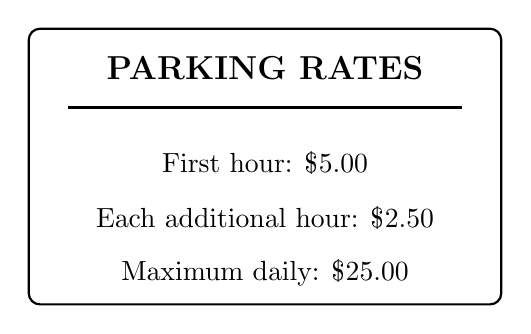
\begin{tikzpicture}
  \draw[thick, rounded corners] (0,0) rectangle (6,3.5);
  \node[font=\bfseries\large] at (3,3) {PARKING RATES};
  \draw[thick] (0.5,2.5) -- (5.5,2.5);
  \node[align=left] at (3,1.8) {First hour: \$5.00};
  \node[align=left] at (3,1.1) {Each additional hour: \$2.50};
  \node[align=left] at (3,0.4) {Maximum daily: \$25.00};
\end{tikzpicture}
\end{center}

Write an expression for the cost of parking for $h$ hours (where $h \geq 1$), and find the cost of parking for $6$ hours.
\end{questionText}
\correctAnswer{$2.50h + 2.50$ (or $5 + 2.50(h-1)$); $\$17.50$}
\explanation{The first hour costs $\$5.00$. Each additional hour costs $\$2.50$, so for $h$ hours the additional hours cost $2.50(h - 1)$. Total: $5 + 2.50(h - 1) = 5 + 2.50h - 2.50 = 2.50h + 2.50$. For $h = 6$: $2.50(6) + 2.50 = 15 + 2.50 = \$17.50$.}
\end{practiceQuestion}

\begin{practiceQuestion}{4-1-q30}{gsa}
\begin{questionText}
The diagram shows a rectangle with the dimensions shown.

\begin{center}
\begin{tikzpicture}[scale=0.8]
  \draw[thick, fill=funBlue!10] (0,0) rectangle (5,3);
  \node[above] at (2.5,3) {$3x + 2$};
  \node[right] at (5,1.5) {$4$};
\end{tikzpicture}
\end{center}

Write an expression for the area of the rectangle, then evaluate it when $x = 3$.
\end{questionText}
\correctAnswer{$12x + 8$; $44$ square units}
\explanation{Area $=$ length $\times$ width $= 4(3x + 2) = 12x + 8$. When $x = 3$: $12(3) + 8 = 36 + 8 = 44$ square units.}
\end{practiceQuestion}
